Měřili jsme hodnoty odporů vytvořených technologií tlusté vrstvy na testovacím substrátu, viz obr.~\ref{fig:img-fuck-png}. Na substrátu byl uvedený motiv 4x a to vždy pootočen o \qty{90}{\degree}, díky takovému měření je pak teoreticky možné stanovit vliv různých parametrů tisku TLV, zejména ověřit, jestli je tisk homogenní v obou osách. Na základě měření je pak možné upravit parametry tisku tak, aby při tisku skutečného integrovaného obvodu byl výsledek co nejvíce optimální a předvídatelný. 

Všechny měřené hodnoty se nachází v tabulce, která je pro lepší přehlednost umístěna až na samotném konci dokumentu. 

\subsection{Zpracování měřených dat}
    Na základě pokynů vyučujícího byla stanovena teoretická hodnota odporu (viz zmíněná tabulka). Vypočtena byla následovně:
    \[
        R_{teor}  = R_{sq}\cdot \frac{L}{W} 
    \]
    Ačkoliv toto nebylo vyučujícím upřesněno, předpokládaná jednotka zadaných rozměrů jsou \unit{\micro\meter}. Z nám dodaných údajů vyplývá, že byla použita odporová pasta s odporem \qty{100}{\ohm\per sq}.

    Následně byla do grafu vynesena závislost odporu na délce rezistoru. Byl vytvořen graf pro každou odporovou sérii a nachází se v něm data ze všech čtyř kvadrantů, pro jednotlivé série se jedná o grafy \ref{graf:RX-1}, \ref{graf:RX-2}, \ref{graf:RX-3} a \ref{graf:RX-4}.

\begin{figure}[h!]
    \centering
    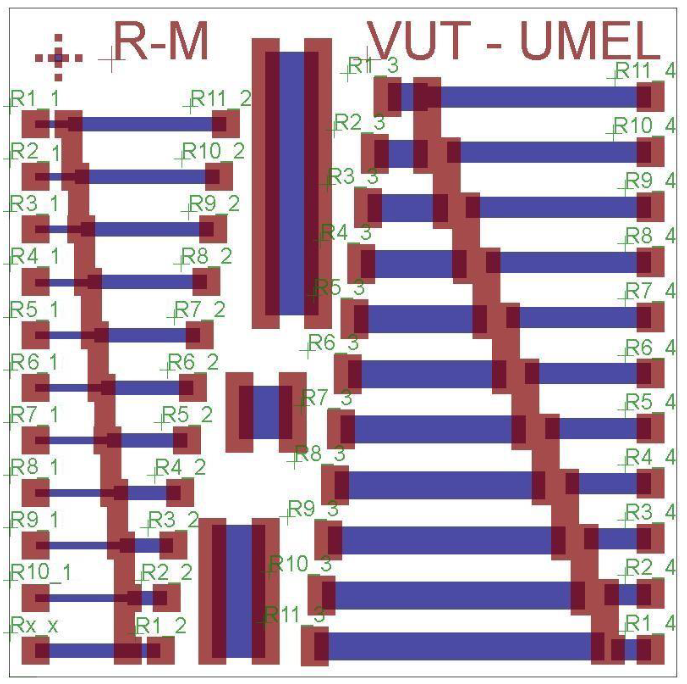
\includegraphics[width=0.5\textwidth]{img/fuck.png}
    \caption{Testovací substrát. Převzato z~\cite{zadani}.}
    \label{fig:img-fuck-png}
\end{figure}

\begin{figure*}[h!]
    \begin{tikzpicture}
        \centering
        \begin{axis}
            [
            xlabel={\( L\ [\unit{\micro\meter}]\)},
            ylabel={\( R\ [\unit{\mega\ohm}]\)},
            %axis y line*=left, % dve y osy
            width=1\textwidth,
            height = 0.5\textwidth,
            legend pos=north west,
%			xmin=0,
%			ymin=0,
%			xmax=100
%			ymax=100
            ]

            \addplot[mark=x, mark options={solid}, thick,  red,   mark size=3pt] table [skip first n=0, x=delka,   y=Q1, col sep=comma] {data/ser1.csv};
            \addlegendentry{RX\_1 Q1}
            \addplot[mark=x, mark options={solid}, thick,  green, mark size=3pt] table [skip first n=0, x=delka, y=Q2, col sep=comma] {data/ser1.csv};
            \addlegendentry{RX\_1 Q2}
            \addplot[mark=x, mark options={solid}, thick,  blue,  mark size=3pt] table [skip first n=0, x=delka,  y=Q3, col sep=comma] {data/ser1.csv};
            \addlegendentry{RX\_1 Q3}
            \addplot[mark=x, mark options={solid}, thick,  black, mark size=3pt] table [skip first n=0, x=delka, y=Q4, col sep=comma] {data/ser1.csv};
            \addlegendentry{RX\_1 Q4}
            
            
        \end{axis}   
    \end{tikzpicture}
    \caption{Závislost odporu na délce. Série RX\_1.}
    \label{graf:RX-1}
\end{figure*}

\begin{figure*}[h!]
    \begin{tikzpicture}
        \centering
        \begin{axis}
            [
            xlabel={\( L\ [\unit{\micro\meter}]\)},
            ylabel={\( R\ [\unit{\mega\ohm}]\)},
            %axis y line*=left, % dve y osy
            width=1\textwidth,
            height = 0.5\textwidth,
            legend pos=north west,
%			xmin=0,
%			ymin=0,
%			xmax=100
%			ymax=100
            ]

            \addplot[mark=x, mark options={solid}, thick,  red,   mark size=3pt] table [skip first n=0, x=delka,   y=Q1, col sep=comma] {data/ser2.csv};
            \addlegendentry{RX\_2 Q1}
            \addplot[mark=x, mark options={solid}, thick,  green, mark size=3pt] table [skip first n=0, x=delka, y=Q2, col sep=comma] {data/ser2.csv};
            \addlegendentry{RX\_2 Q2}
            \addplot[mark=x, mark options={solid}, thick,  blue,  mark size=3pt] table [skip first n=0, x=delka,  y=Q3, col sep=comma] {data/ser2.csv};
            \addlegendentry{RX\_2 Q3}
            \addplot[mark=x, mark options={solid}, thick,  black, mark size=3pt] table [skip first n=0, x=delka, y=Q4, col sep=comma] {data/ser2.csv};
            \addlegendentry{RX\_2 Q4}
            
            
        \end{axis}   
    \end{tikzpicture}
    \caption{Závislost odporu na délce. Série RX\_2.}
    \label{graf:RX-2}
\end{figure*}

\begin{figure*}[h!]
    \begin{tikzpicture}
        \centering
        \begin{axis}
            [
            xlabel={\( L\ [\unit{\micro\meter}]\)},
            ylabel={\( R\ [\unit{\mega\ohm}]\)},
            %axis y line*=left, % dve y osy
            width=1\textwidth,
            height = 0.5\textwidth,
            legend pos=north west,
%			xmin=0,
%			ymin=0,
%			xmax=100
%			ymax=100
            ]

            \addplot[mark=x, mark options={solid}, thick,  red,   mark size=3pt] table [skip first n=0, x=delka,   y=Q1, col sep=comma] {data/ser3.csv};
            \addlegendentry{RX\_3 Q1}
            \addplot[mark=x, mark options={solid}, thick,  green, mark size=3pt] table [skip first n=0, x=delka, y=Q2, col sep=comma] {data/ser3.csv};
            \addlegendentry{RX\_3 Q2}
            \addplot[mark=x, mark options={solid}, thick,  blue,  mark size=3pt] table [skip first n=0, x=delka,  y=Q3, col sep=comma] {data/ser3.csv};
            \addlegendentry{RX\_3 Q3}
            \addplot[mark=x, mark options={solid}, thick,  black, mark size=3pt] table [skip first n=0, x=delka, y=Q4, col sep=comma] {data/ser3.csv};
            \addlegendentry{RX\_3 Q4}
            
            
        \end{axis}   
    \end{tikzpicture}
    \caption{Závislost odporu na délce. Série RX\_3.}
    \label{graf:RX-3}
\end{figure*}

\begin{figure*}[h!]
    \begin{tikzpicture}
        \centering
        \begin{axis}
            [
            xlabel={\( L\ [\unit{\micro\meter}]\)},
            ylabel={\( R\ [\unit{\mega\ohm}]\)},
            %axis y line*=left, % dve y osy
            width=1\textwidth,
            height = 0.5\textwidth,
            legend pos=north west,
%			xmin=0,
%			ymin=0,
%			xmax=100
%			ymax=100
            ]

            \addplot[mark=x, mark options={solid}, thick,  red,   mark size=3pt] table [skip first n=0, x=delka,   y=Q1, col sep=comma] {data/ser4.csv};
            \addlegendentry{RX\_4 Q1}
            \addplot[mark=x, mark options={solid}, thick,  green, mark size=3pt] table [skip first n=0, x=delka, y=Q2, col sep=comma] {data/ser4.csv};
            \addlegendentry{RX\_4 Q2}
            \addplot[mark=x, mark options={solid}, thick,  blue,  mark size=3pt] table [skip first n=0, x=delka,  y=Q3, col sep=comma] {data/ser4.csv};
            \addlegendentry{RX\_4 Q3}
            \addplot[mark=x, mark options={solid}, thick,  black, mark size=3pt] table [skip first n=0, x=delka, y=Q4, col sep=comma] {data/ser4.csv};
            \addlegendentry{RX\_4 Q4}
            
            
        \end{axis}   
    \end{tikzpicture}
    \caption{Závislost odporu na délce. Série RX\_4.}
    \label{graf:RX-4}
\end{figure*}
